\documentclass{article}


\usepackage{arxiv}

\usepackage[utf8]{inputenc} % allow utf-8 input
\usepackage[T1]{fontenc}    % use 8-bit T1 fonts
\usepackage{hyperref}       % hyperlinks
\usepackage{url}            % simple URL typesetting
\usepackage{booktabs}       % professional-quality tables
\usepackage{amsfonts}       % blackboard math symbols
\usepackage{nicefrac}       % compact symbols for 1/2, etc.
\usepackage{microtype}      % microtypography

% Packages that are not related to the template
\usepackage{natbib}
\usepackage{graphicx}
\usepackage{amsthm}
\usepackage{amsmath}
\usepackage{systeme}
\usepackage{algorithmic}
\usepackage[thinc]{esdiff}

\graphicspath{ {./images/} }

\newtheorem{definition}{Definition}

\title{Optimal liquidation strategy in a mixed call auction and continuous auction market}

\author{
 Hoang Hai Tran\\
 Department of Statistics \& Applied Probability\\
 National University of Singapore \\
 Lower Kent Ridge Road 10 \\
 119076 Singapore \\
 \texttt{e0045275@nus.edu.sg} \\
   \And
 Ying Chen\\
 Department of Mathematics and Risk Management Institute \\
 National University of Singapore \\
 Lower Kent Ridge Road 10 \\
 119076 Singapore \\
 \texttt{matcheny@nus.edu.sg} \\
}

\begin{document}
\maketitle

\begin{abstract}
  We analyze the price impact of trading in a mixed auction market, in which the exchange employs both call auction and continuous auction. Based on a multiplayer game settings between a market maker and one or many liquidity takers, we derive a market impact model characterizes both instantaneous and temporary price impact. Our first main result is an unified model of how price discovery and market impact transition from call auction to the continuous auction. Our second main result is that, based on our market impact model, there is an optimal trading strategy with closed-form solution to liquidate a portfolio under both auctions. We furthermore analyze the optimal trading strategy numerically to show the cost efficiency of trading in both auctions compared to trading only in continuous trading auction.
\end{abstract}

\section{Introduction}
In modern financial markets, double auction is a standard process of buying and selling shares with multiple sellers and multiple buyers. From an economist's perspective, an auction can be considered a price discovery process, where a competitive equilibrium price is found through interactions among bidders. The price is usually assumed to be the point where supply and demand are equal. The question of how the price reaches its equilibrium points, and how different players use their own information advantages to achieve a preferable price, has attracted researchers from various fields. \cite{Kyle1985} studies how market makers, insider traders and noise traders interact to form an equilibrium price in a continuous trading auction. \cite{AlmgrenChriss2000} discusses how execution can be done optimally in a continuous trading phase under certain market impact assumptions. \cite{Avellaneda2008} derives an equilibrium price from the perspectives of a market maker to provide quotes in a continuous trading auction. This paper is in a similar vein, in which we discuss how price will reach its equilibrium price in a mixed auction market. By taking into account call auction, under different market impact assumptions, we derive the corresponding optimal liquidation strategy for a trader to unwind his position. We provide theoretical evidence that it is indeed cheaper to trade the call auction compared to the continuous auction. Specifically, we examine the impact of trading in a market that operates under two auction models:
\begin{itemize}
  \item \textbf{Call auction} Buyers set a maximum price that they want to buy, and sellers set a minimum price that they want to sell. The orders will then be batched together and matched at a price set by the exchange.
  \item \textbf{Continuous auction} Orders are matched continuously based on time and price priority. Participants in the auction can choose to either queue their orders to wait for an opposing trade, or cross the book to match against other's orders.
\end{itemize}

Historically, the debate of whether the call auction is required along with the continuous auction in the financial market started with the adoption of electronic trading. The transition from manual to automatic trading system around the world began from the early 80s to the late 90s, with Toronto (1977) being the first exchange to implement an electronic matching system. Other exchanges soon followed, including Tokyo (1982), Paris (1986) and Germany (1991). By the end of the 20th century, major exchanges around the world have shifted to electronic trading. Initially, exchanges operate in favor of a continuous trading market, in which orders are matched instantly through out the day. Continuous trading was deemed most suitable for electronic trading because participants can transact immediately. However, as argued in (\cite{Economides1995}), a call auction may be preferred over a continuous trading auction under certain circumstances. Consequently, most exchanges around the world implemented call auction sessions in addition to the continuous trading session. By 2020, major exchanges around the world implement mixed auction mechansim with an opening call auction, followed by a continuous trading session and end the day with a closing call auction.

The adoption of the call auctions has resulted in substantial shift of daily trading activity, with the call auctions responsible for a significant proportion of the average daily trading volumes. (\cite{Madhavan2015}) found that the call auction in New York Stock Exchange (NYSE) accounts for roughly 10 percent of the average trade value. (\cite{Bruno1999}) found similar phenomenon on the Paris Bourse, in which the opening auction accounts for about 10 percent of average daily trade value. (\cite{Carole2006}) has a similar conclusion regarding the Australian Stock Exchange (ASX).

A call auction can lower execution costs for participants and improve price discovery process, as suggested in (\cite{Pagano2003}). The reduction in trading costs, such as market impact and adverse selection costs, is achieved through several channels, including (\cite{Carole2006}):

\begin{itemize}
  \item Temporal consolidation of order flow and execution of orders at a single price (\cite{Economides1995}).
  \item Facilitation of price discovery process during times of market stress (\cite{Madhavan1992}).
\end{itemize}

Various studies have found that there are significant strategic trading activities during the call auctions. (\cite{Bruno1999}) suggests that the fluctuation in the indicative price during the call auction period maybe due to strategic trading. (\cite{Vives2001}) argues that large market makers may have incentives to trade during the opening call auction, to mitigate information leakage.

On the other hand, literature on optimal liquidation and market impact has rarely mentioned execution during call auctions, not to mention the mixed auction environment. One of the first study on optimal liquidation is (\cite{HoStoll1981}), in which an optimal trading curve is derived under certain assumptions on stochastic trade arrival and price process. (\cite{AlmgrenChriss2000}) extends the model further by incorporating a trader's risk aversion factor when pricing for an optimal liquidation strategy. (\cite{Obizhaeva2013}) solves the problem under a different assumption: the impact of each trade recovers slowly instead of immediately. These works are derived for continuous auction. In terms of trading during a call auction, (\cite{Madhavan2015}) derives a optimal liquidation strategy for a specialist to set an equilibrium price under the assumptions of multiple traders with private information.

Works on optimal execution today focuses more on minimizing the impact of trading during the continuous trading phase, which ignores the fact that the opening auction is usually very liquid and the matched volume represents a significant portion of daily trading volume. For executing a big block order with significant volume, including call auctions are usually more preferable since the execution cost is lower, as shown in our analysis later. Specifically, based on our theoretical framework, we found that:

\begin{itemize}
  \item There is a potentially large gain from liquidating portion of the position in the call auction, since the call auction provides another venue to take liquidity from.
  \item Due to inventory management from the market maker, the transition period from the call auction will be characterized with a wide initial spread that will narrow over time. A mixed auction strategy takes into account this effect will reduce transition cost even further.
  \item There is an optimal liquidation strategy to execute trade during both the call auction and the continuous auction that results in better cost optimization than trading in the continuous auction only.
\end{itemize}

This paper is organized as follows: Section (\ref{sec:AnalyticalFramework}) will present the theoretical framework that we will use to characterize the call auction and optimize our trading strategy. Section (\ref{sec:EmpiricalAnalysis}) will perform empirical analysis based on the theoretical framework to examine their effects on the optimal trading strategy and its cost efficiency. Section (\ref{secConclusion}) will conclude the paper with suggestions for further research.

\section{The Analytical Framework}\label{sec:AnalyticalFramework}

In order to derive an optimal liquidation strategy in a mixed auction market, we must first specify the auction mechanism for each session and how trading will impact the fair price of the market. We consider a market with two trading sessions in succession: a call auction session and a continuous trading session. The mechanism of each session, number of participants in each session and how their interaction affects the price of the underlying risky asset will be described, following by the market impact formula and the optimal liquidation strategy.

\subsection{Call auction mechanism and agents' behaviours}\label{subsec:AnalyticalFrameworkCallAuction}

In this section we will examine how different participants contribute to the price discovery process during the call auction. We assume the call auction is fully automated, and the matching mechanism is modelled after a Walrasian auction. Traders can submit and amend orders anytime during the call auction. Those orders are not matched immediately, and placed into the book as "crossed", that is, the highest buy price is higher than the lowest sell price in the book (see Table (\ref{itayoseTable1}) for an example book during the call auction). At the end of the auction period, the orders in the book are matched based on an equilibrium price calculated by the exchange. The equilibrium price is determined to maximize the volume traded in the call auction, and therefore has to satisfy the following requirements:

\begin{itemize}
  \item All buy/sell orders at prices higher/lower than the equilibrium price must be executed.
  \item At the execution price, the entire either buy or sell quantity must be matched.
\end{itemize}

Table (\ref{itayoseTable2}) gives an example of how a book can be "un-crossed" at the end of the call auctions. All the orders that are unmatched at the end of the call auction will be transferred to the continuous trading session. There is no specialist who can step in to modify the equilibrium price. This mechanism is adopted for the opening call auctions in Singapore Stock Exchange (SGX), Tokyo Stock Exchange (TSE) and Nasdaq Stock Market (NASDAQ). New York Stock Exchange (NYSE) is different, in which a specialist sets the equilibrium price that is not necessarily the same as the volume-maximizing Walrasian price.

\begin{table}[]
  \centering
  \begin{tabular}{c|c|c|c|c}
    \hline
    \textbf{Total Buy} & \textbf{Buy} & \textbf{Price} & \textbf{Sell} & \textbf{Total Sell} \\ \hline
                       &              & 56             & 4000          & 16100               \\ \hline
                       &              & 55             & 10000         & 12100               \\ \hline
    3000               & 3000         & 54             & 2000          & 2100                \\ \hline
    3100               & 100          & 53             & 100           & 100                 \\ \hline
    7100               & 4000         & 52             &               &                     \\ \hline
    10100              & 3000         & 53             &               &                     \\ \hline
  \end{tabular}

  \caption{A sample crossed orderbook during call auction. The orders will be matched at the equilibrium price of 54, which results in 2100 shares traded.}
  \label{itayoseTable1}
\end{table}


\begin{table}[]
  \centering
  \begin{tabular}{c|c|c|c}
    \hline
    \textbf{Buy} & \textbf{Price} & \textbf{Sell} & \textbf{Trade} \\ \hline
                 & 56             & 4000          &                \\ \hline
                 & 55             & 10000         &                \\ \hline
    900          & 54             &               & 2100           \\ \hline
    100          & 53             &               &                \\ \hline
    4000         & 52             &               &                \\ \hline
    3000         & 53             &               &                \\ \hline
  \end{tabular}
  \caption{A sample orderbook at the end of the call auction.}
  \label{itayoseTable2}
\end{table}

Inspired by the framework in (\cite{Madhavan2015}), we model the call auction as a two-stage game. Orders are submitted by all participants in first stage of the game, during the call auction period. In the second stage, the book is matched based on the Walrasian price described above. We assume that there are two types of participants:

\begin{itemize}
  \item Market markers are those with private information about the value of the asset. This information is not necessary from possessing some insider knowledge about the asset, but from having access to superior information regarding the order flow of the book, such as real-time trades and quotes provided by the exchange and better data processing capability.
  \item Liquidity traders are those without private information and simply want to execute their orders. We assume the demands of liquidity traders are exogenous, and they trade using market orders.
\end{itemize}

Unlike (\cite{Madhavan2015}), we do not assume that there is a specialist setting the equilibrium price, as most exchanges around the world has adopted automated call auction mechanism at the time of this writing. We also do not assume that there are informed traders with information advantage, but a market maker who holds private information and make the market instead. There are several reasons for this setup:
\begin{itemize}
  \item The model setup assumes that, in order to fully utilize the information advantage, the participant who holds it must have the ability to reprice his orders immediately after he receives a new signal. As we assume the private information is mainly from observing the order flow of the book, it means the participant is a high frequency trader (HFT), who can act immediately after each change in market order flow.
  \item There are evidences that a significant portion of high frequency trading during is for liquidity provision. (\cite{Menkveld2013}) studied the trading activity in Chi-X Europe, and found that a majority of high frequency trading activities is market making. Similarly, \cite{Bellia2017} found that there is a correlation between low-latency trading and the subsequent liquidity provision in the call auction in Tokyo Stock Exchange (TSE).
\end{itemize}

We further assume that there is a single market maker who makes the market for $K$ liquidity traders. This can be either a designated market maker obligated to provide liquidity for the market, or an external agent who wants to capture the liquidity premium of the call auction. The market maker is then assumed to have a negative exponential expected utility function of the form
\[
  u(W_e) = -e^{-\lambda W_e}
\]
where $W$ is the terminal wealth of the trader at the end of the call auction. The terminal wealth of the market maker is
\[
  W_e = p_0 (q + e_e) + (c_e - p_e q)
\]
The notions are
\begin{itemize}
  \item $\lambda>0$ is the risk aversion factor of the market maker.
  \item $p_0$ is the stock's fair price at the end of the call auction.
  \item $p_e$ is the stock's equilibrium price at the end of the call auction.
  \item $c_e$ is the initial cash position of the market maker.
  \item $e_e$ is the overnight position of the market maker.
  \item $q$ is number of shares purchased by the market maker at the end of the call auction.
\end{itemize}
To model the asset price at the end of the call auction, we assume that the asset value $p_0$ follows normal distribution with mean $\mu_e$ and precision (the inverse of the variance) $\zeta_e$ \footnote{While this means the stock may have negative price as time goes by, we can ignore this risk as we only need to account for one day of variance. Using an arithmetic stock price process instead of the classical logarihmic price process simplifies other calculation later in the study.}. The private information of market maker $\omega_e$ is then the normal variable
\[
  \omega_e \sim N(p_0, \frac{1}{\psi_e})
\]
The posterior distribution of the asset according to market maker's information set $\Omega_e$ is then normally distributed with mean
\[
  p_0=E[p_0|\Omega_e]=\mu_e \alpha + \omega_e(1 - \alpha)
\]
where
\[
  \alpha = \frac{\zeta_e}{\zeta_e+\psi_e}
\]
and variance
\[
  \sigma_e^2=var[v|\Omega_e]=\frac{1}{\zeta_e+\psi_e}
\]
Maximizing expected utility of the market maker, we have the amount of shares submitted
\begin{equation}\label{eqn:mm_eval_eqb}
  q(p) = a_e - b_e p
\end{equation}
where $a_e = \frac{p_0}{\lambda \sigma_e^2} - e_e$ and $b_e=\frac{1}{\lambda \sigma_e^2}$. We assume the $K$ liquidity traders will submit a total of $\sum_{i=0}^K x_i$ shares into the call auction to be matched, with negative values implying selling and vice versa. The total shares transacted at a given price $p$ is then
\[
  Q(p) = (p_0 - p) b_e + \sum_{i=0}^K x_i
\]
At equilibrium, we set $Q(p)$ to 0. This gives the Walrasian price as the matching price at the end of the call auction
\begin{equation}\label{markup_px_eqb}
  p_e = p_0 + \frac{\sum_{i=0}^K x_i}{b_e}
\end{equation}
The matching price is the fair price of the stock with a mark-up in proportion to the supply-demand imbalance in the market. The pricing function is plotted in Figure (\ref{fig:mm_pricing_auction}), which we will use to price our market impact of trading with the call auction in subsection (\ref{subsec:AnalyticalFrameworkTransitionPeriod}) after we examine the continuous trading phase in the next section.

\begin{figure}[h]
  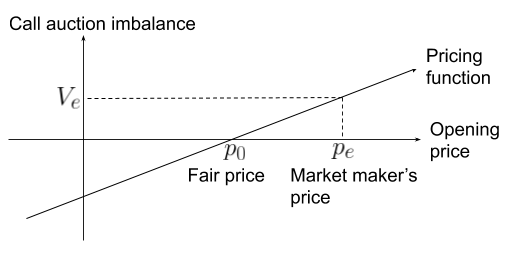
\includegraphics[width=\textwidth]{MMPricing}
  \caption{Pricing function of the market maker w.r.t call auction imbalance. If the imbalance is negative, implying that the sell demand is higher than buy demand, the market maker will price the opening price to be lower than his fair price, and vice versa. The slope of the pricing function is $\frac{1}{b_e}$ in Equation (\ref{markup_px_eqb}). $V_e$ is the imbalance at the end of the call auction, while $p_e$ is the opening price. }
  \label{fig:mm_pricing_auction}
\end{figure}

\subsection{Continuous auction mechanism and agents' behaviours}\label{subsec:AnalyticalFrameworkContinuousAuction}
During the continuous trading session, orders can be posted into the market at anytime during the session and will be matched immediately. If a buy order has a price that is higher than the current lowest offer in the book, it will be matched immediately, and vice versa for sell orders. Otherwise, they will be added into the book.

Similar to the call auction, we model the continuous auction as a multi-round two-stage game. At the beginning of each round, we pick randomly a liquidity trader to act as the counterparty of the market maker. In the first stage of the round, the market maker place limit orders in the book according to his risk tolerance and private information. In the second stage, the liquidity trader will place a market order based on his exogenous demand. This setup is slightly different from the call auction in which:
\begin{itemize}
  \item Unlike the call auction, only the market maker can submit limit orders during the first stage of the game. He has no knowledge of the liquidity trader's order, and only submit orders based on his own evaluation of the asset's value.
  \item The liquidity trader can only submit market orders during the final stage of the game, after the market maker has finished layering his orders in the book.
\end{itemize}
Under this mechanism, the market maker has a speed advantage with respect to the rest of the market, since he can evaluate the current fair pricing of the asset after each trade. After the reevaluation, he can modify his orders in the market to reflect the updated belief before any liquidity traders can place a new order. This grants the market maker distinct competitive advantage, in the sense that he can reprice his orders in the book before getting hit by any adverse selection event. This gives incentive to market makers to perform high frequency trading.

Similar to the call auction, we assume the market maker has private information about the asset from his superior analytical capability. Again, let assume the immediate asset value at the end of the continuous auction's round is a random variable $v_c$ normally distributed with mean $\mu_c$ and precision $\zeta_c$. The market maker deduces his own evaluation with a private signal
\[
  \omega_c \sim N(v_c, \frac{1}{\zeta_c})
\]
and forms a posterior belief on the asset value at the end of the round as a normal random variable with mean
\[
  v_c=\mu_c \alpha + \omega_c(1 - \alpha)
\]
where
\[
  \alpha = \frac{\zeta_c}{\zeta_c+\psi_c}
\]
and variance
\[
  \sigma_c^2=\frac{1}{\zeta_c+\psi_c}
\]

At the beginning of each round, the market maker has a position $e_c$ that he wants to liquidate. Maximizing the market maker's utility function, we have his order quantity function in the book:
\begin{equation}\label{eqn:mm_eval_cont}
  q_c(p) = a_c - b_c p_c
\end{equation}
where $a_c = \frac{v_c}{\lambda \sigma_c^2} - e_c$ and $b_c=\frac{1}{\lambda \sigma_c^2}$. Let assume the liquidity trader needs to transact $x_0$ shares. The average price he gets after submitting his market order is
\[
  p_{avg} = \frac{a_c-x_0}{b_c}=p_0 - \frac{1}{b_c} x_0
\]
where
\[
  p_0 = \frac{a_c}{b_c}
\]
is the best price quoted by the market maker. Note that the position is from the perspective of the market maker, that is, the higher number of shares the liquidity trader wants to buy, the higher markup price he will have to pay to transact immediately. In other words, the markup price that the liquidity trader receives is
\begin{equation}\label{eqn:markup_px_cont}
  p_{avg} = p_0 + \frac{1}{b_c} x_0
\end{equation}

Comparing Equation (\ref{markup_px_eqb}) and Equation (\ref{eqn:markup_px_cont}), we can see that, ceteris paribus, the instantaneous market impact of trading during the auction phase has a higher chance of getting offset by other liquidity traders in the market. On the other hand, during the continuous phase, the liquidity trader will always receive an adverse markup price implied in market maker's quotes. This is clearer once we examine the transition period immediate after market opening in the next subsection.

\subsection{Price discovery at market opening}\label{subsec:AnalyticalFrameworkTransitionPeriod}

There are empirical evidence that the transition period immediate after market opening is crucial in determining the effectiveness of the opening call auction (\cite{Pagano2013}). In this subsection, we analyze how the market maker, and consequently the spread, may behave during this period, and the subsequent effects on the liquidity trader. Recalling from Equation (\ref{markup_px_eqb}), the opening price is marked up proportional to the buy-sell imbalance at the end of call auction. Let
\[
  V_e = \sum_{i=0}^K x_i
\]
be the imbalance at the end of call auction. Based on the imbalance, the market maker will provide the liquidity necessary for the market to open at price
\[
  p_e = p_0 + \frac{V_e}{b_e}
\]
Without loss of generality, let $V_e$ be positive, implying that the market has more buy interests than sell interests. The market maker will sell $V_e$ shares at price $p_e$ higher than his estimated fair value of $p_0$, and has an unrealized gain of
\[
  G_e = (p_0 - p_e) * V_e
\]
To capitalize this gain after market opening, the market maker will need to make a spread. Continuing from the call auction's we have the pricing function of the market maker during this period:
\[
  q(p) = a_e - b_e p
\]
where $a_e = \frac{p_0}{\lambda \sigma_e^2} - V_e$ and $b_e=\frac{1}{\lambda \sigma_e^2}$, based on his signal when pricing the call auction. As $V_e$ is positive, this means the market maker is willing to sell at $p_e$. On the other hand, it is reasonable to assume that he will want to liquidate his position acquired from the opening call auction at $p_0$, his fair price of the asset at the end of the call auction. Therefore, the market maker will make a spread of $\frac{V_e}{b_e}$ immediately after call auction. The quotes of the market maker are illustrated in Figure (\ref{fig:mm_pricing_transition}).

\begin{figure}[h]
  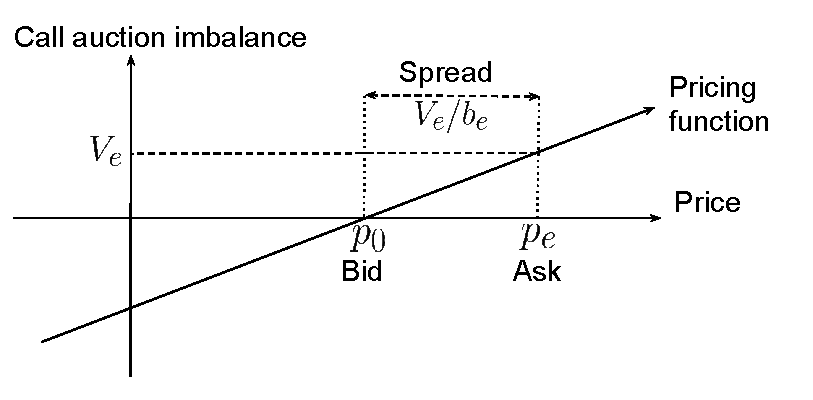
\includegraphics[width=\textwidth]{MMPricingTransition}
  \caption{Market maker's quotes immediately after opening w.r.t call auction imbalance. Upon market opening, the market maker will short $V_e$ shares at $p_e$. His evaluation of the asset's fair value is at $p_0$. However, due to his inventory, he will quote the ask side further away at $p_e$, and bid side at $p_0$. The bid-ask spread is then $\frac{V_e}{b_e}$, based on the market maker's pricing function (\ref{eqn:markup_px_cont}).}
  \label{fig:mm_pricing_transition}
\end{figure}

Interestingly, the bid-ask spread after market opens reveals the market maker's pricing in the call
auction, as we can calculate the implicit factor $b_e$ as
\begin{equation}\label{eqn:expected_spread}
  b_e = \frac{V_e}{\zeta_e}
\end{equation}
where
\begin{itemize}
  \item $V_e$ is the matching volume at the open of continuous trading session.
  \item $\zeta_e$ is the spread at the open of continuous trading session.
\end{itemize}

From the similarity of the pricing function during the call auction in Equation (\ref{markup_px_eqb}) and the continuous auction in Equation (\ref{eqn:markup_px_cont}), we can see that, ceteris paribus, it is advantageous to trade in both sessions to consume liquidity from both to lower his market impact. This will become clearer once we derive the optimal trading strategy in the next section. Moreover, as the call auction compresses the liquidity over a long period in one single price, there is usually a larger than normal amount of shares matched that the market marker will need to unwind during the transition period. This will affect the pricing for the liquidity trader during this period, in addition to the normal pricing in the continuous session. Specifically, the liquidity trader will potentially face one of the following two scenarios during the call auction:

\begin{itemize}
  \item {\textbf{Scenario 1: The liquidity trader trades in the same direction as the market imbalance}
        As $V_e$, the buy-sell imbalance at the end of the call auction, is assumed to be positive, we have the liquidity trader wants to buy in this case. As a result, his block trade size of $B_0$ will push the opening ask up, from $p_e$ to
        \[
          p_{e+} =  p_0 + \frac{V_e + B_0}{b_e}
        \]
        As he is buying, this is equivalent to lifting the offer during the continuous phase. In this case, ceteris paribus, there is no difference between trading during the auction and trading during the continuous phase.

        \begin{figure}[h]
          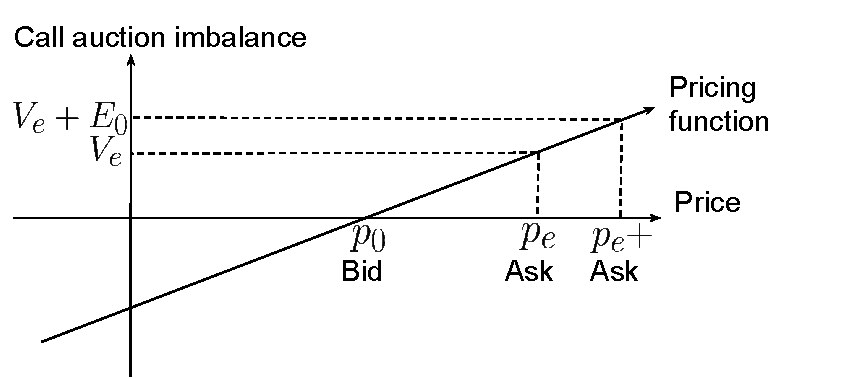
\includegraphics[width=\textwidth]{MMPricingTransitionSameDir}
          \caption{Bid-ask spread under Scenario 1, in which the liquidity trader trades in the same direction as the bid-ask imbalance. Consequently, he will push the ask price up, increase the cost of trading both in the call auction and the subsequent continuous phase.}
          \label{fig:mm_pricing_transition_s1}
        \end{figure}
        }
  \item {
        \textbf{Scenario 2: The liquidity trader trades against the market imbalance}
        In this case, the liquidity trader will sell to the market, similar to the market maker. Therefore, he is providing liquidity to the market, reducing the bid-ask spread immediately after market opening. In other words, the opening price bid improves from $p_e$ to
        \[
          p_{e-} = p_0 + \frac{V_e - B_0}{b_e}
        \]
        As he is selling, this is equivalent to placing his offer into the bid-ask spread during the continuous phase and getting filled immediately.
        \begin{figure}[h]
          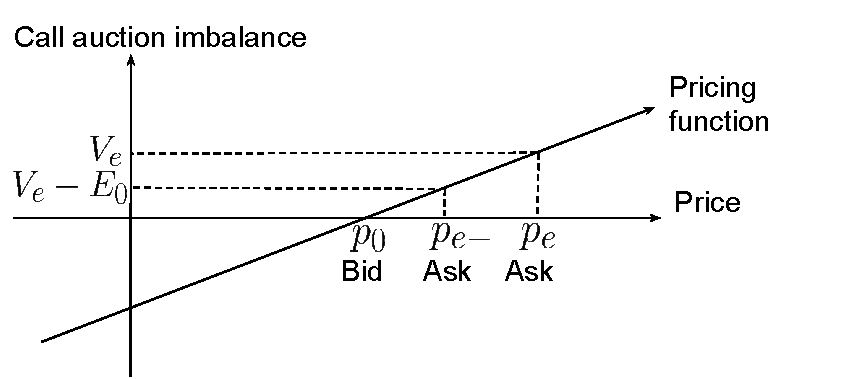
\includegraphics[width=\textwidth]{MMPricingTransitionDifferentDir}
          \caption{Bid-ask spread under Scenario 2, in which the liquidity trader trades against the bid-ask imbalance. Consequently, he will pull the opening ask price down, while leave the opening bid at $p_0$. As he is selling, there is no impact on his cost of trading after market opening.}
          \label{fig:mm_pricing_transition_s2}
        \end{figure}
        }
\end{itemize}
As the market maker is buying at the fair price of $p_0$ and selling at a discounted price $p_e$, it is reasonable that he will get filled more on the bid side than the ask side.

\begin{itemize}
  \item Under Scenario 1, trading in the call auction results in an ongoing penalty cost to the liquidity trader that will decay over time, as he will need to lift the offer to sell. Let the speed of liquidation of the market maker be $\rho$ and $V_t$ be the remaining position of the market maker acquired from the call auction in Scenario 1. Consequently, we have
        \[
          dV_t = -\rho V_t
        \]
        \[
          V_t[0]=(V_e + B_0)
        \]
        \begin{equation}\label{eqn:recovery_term_eqb}
          \Leftrightarrow V_t = (V_e + B_0) e^{-\rho t}
        \end{equation}
        where $B_0$ is the liquidity trader's block trade size during auction. The resulting spread due to our trading during the call auction at time $t$ will be
        \begin{equation}\label{resilence_term}
          \zeta_t = \frac{e^{-\rho t}}{b_e}  (V_e + B_0)
        \end{equation}

        Therefore, we would expect the spread to be wide initially, and slowly closing due to the inventory management effects from the market maker. This is in agreement with current empirical evidence that the bid-ask spread narrows shortly after market opens.
  \item Under Scenario 2, trading in the call auction has no "spillover" effect on the liquidity trader, as the liquidity trader will keep hitting the bid to sell while the market maker will try to improve the offer.
\end{itemize}

As this "spillover" cost only happens half of the time, under Scenario 1, the markup cost to the liquidity trader during this transition period is:

\begin{equation}\label{resilence_term}
  \zeta_t = \frac{e^{-\rho t}}{2 b_e}  (V_e + B_0)
\end{equation}
which we use in the next section to derive the optimal liquidation strategy for the liqudity trader.

\subsection{Optimal liquidation strategy in a mixed auction market}

Based on the behaviors of market makers in the previous subsections, we can derive the market impact of trading for the liquidity trader in each of the session. Suppose the fundamental price process $S_t$ at time $t$ is given by
\[
  S_t = S_0 + \int_0^t \sigma dZ_s
\]
that is, $S_t$ follows a classical arithmetic random walk without any drift. The actual price process $P_t$ is then the combination of the fundamental price process $S_t$ and a short term deviation process $D_t$ due to the market maker repricing his book, as described in Subsection (\ref{subsec:AnalyticalFrameworkCallAuction}) and (\ref{subsec:AnalyticalFrameworkContinuousAuction}):

\[
  P_t = S_t + D_t
\]

From Equation (\ref{markup_px_eqb}) and Equation (\ref{eqn:markup_px_cont}), it is reasonable to assume that $D_t$ will include a linear cost component proportional to the trading sizes under each session:
\begin{equation}\label{short_term_deviation}
  D_t = \alpha B_0 + E_t \beta
\end{equation}
where
\begin{itemize}
  \item $B_0$ is the block trade size at the end of the call auction
  \item $E_t$ is the continuous trading rate of the liquidity trader
  \item $\alpha$ and $\beta$ are the cost penalty factor for aggressing the book during the call auction and continuous auction, respectively. We have $\alpha=\frac{1}{b_e}$ and $\beta=\frac{1}{b_c}$ based on Equation (\ref{markup_px_eqb}) and Equation (\ref{eqn:markup_px_cont}), respectively.
\end{itemize}
Equation (\ref{short_term_deviation}) is similar to what has been described as the "temporary impact" term in in the pioneering works of (\cite{BertimasLo1999}) and (\cite{AlmgrenChriss2000}). On the other hand, from Equation (\ref{resilence_term}), we have the expected spillover cost of trading during call auction to continuous phase is:
\[
  R_t = \frac{\alpha (B_0 + \bar{V_e}) e^{-\rho t}}{2}
\]

The short term deviation term $D_t$ is then
\[
  D_t = \underbrace{\alpha B_0 }_\text{Cost of aggressing the book at the end of the call auction} +
  \underbrace{\frac{\alpha (B_0 + \bar{V_e}) e^{-\rho t}}{2}}_\text{Spillover cost from call auction} +  \underbrace{\beta E_t}_\text{Cost of aggressing the book during continuous auction}
\]
and the market impact cost of trading is
\begin{equation}\label{eqn:cost_equation_all}
  C_t = \alpha B_0^2 + \int_0^t \frac{\alpha (B_0 + \bar{V_e}) e^{-\rho t}}{2} E_s ds + \int_0^t \beta E_s^2 ds
\end{equation}
which we can use to derive an optimal strategy for the liquidity trader. Let assume the liquidity trader wants to unwind a large position, and he has the option to exercise his trades in both the call auction and the continuous auction. We have the following notations regarding his trading strategy:

\begin{itemize}
  \item $Q_t$ is the total number of shares of his portfolio at time t.
  \item $E_t$ is the continuous liquidation strategy during the continuous trading auction.
  \item $X_t=\int_0^t E_s ds$ is remaining shares at time $t$.
  \item $B_0=Q_0 - \int_0^T E_s ds$ is the size of the block trade executed at the end of the opening call auction.
\end{itemize}

Based on the Proof (\ref{proof:optimal-strategy}) in the Appendix, we have the optimal size of block trade in the call auction is:
\[
  B_0 = \frac{Q_0 F_{11} + V_e F_{12}}{F_2}
\]
where
\[
  F_{11} = 8 e^{T \rho} \beta \rho [\alpha - e^{T \rho} (\alpha - 4 \beta \rho)]
\]
\[
  F_{12} = (e^{T \rho}-1) \alpha [\alpha (2+T \rho) + e^{T \rho} (8 \beta \rho + \alpha (T \rho - 2 ))]
\]
\[
  \begin{split}
    F_2 = \alpha^2 (2 + T \rho) - 4 e^{T \rho} \alpha (\alpha + 2 \beta \rho)
    + e^{2 T \rho} [8 \beta \alpha \rho + 8 \beta (T \alpha + \beta) \rho^2 + \alpha^2 (2 - T \rho)]
  \end{split}
\]
The optimal trading strategy during continuous session is:
\[
  E_t = A - B_0 \frac{\alpha e^{-t \rho}}{4 \beta}
\]
\[
  X_t = A t - B_0 \frac{\alpha (1- e^{-t \rho})}{4 \beta \rho}
\]
where
\[
  A =   \frac{4 (Q_0 - B_0) + \frac{(1 - e^{-T \rho})}{\beta \rho} B_0 \alpha} {4 T}
\]
The optimal trading strategy during auction phase is a combination of a TWAP with an exponentially decayed component to account for the spillover effect. A sample optimal allocation between the auction's block trade and the continuous trading strategy's size is in Figure (\ref{fig:optimal_sizes}). The corresponding optimal liquidation rate curve of the strategy is plotted in Figure (\ref{fig:optimal_curve_strategy}).


\begin{figure}[h]
  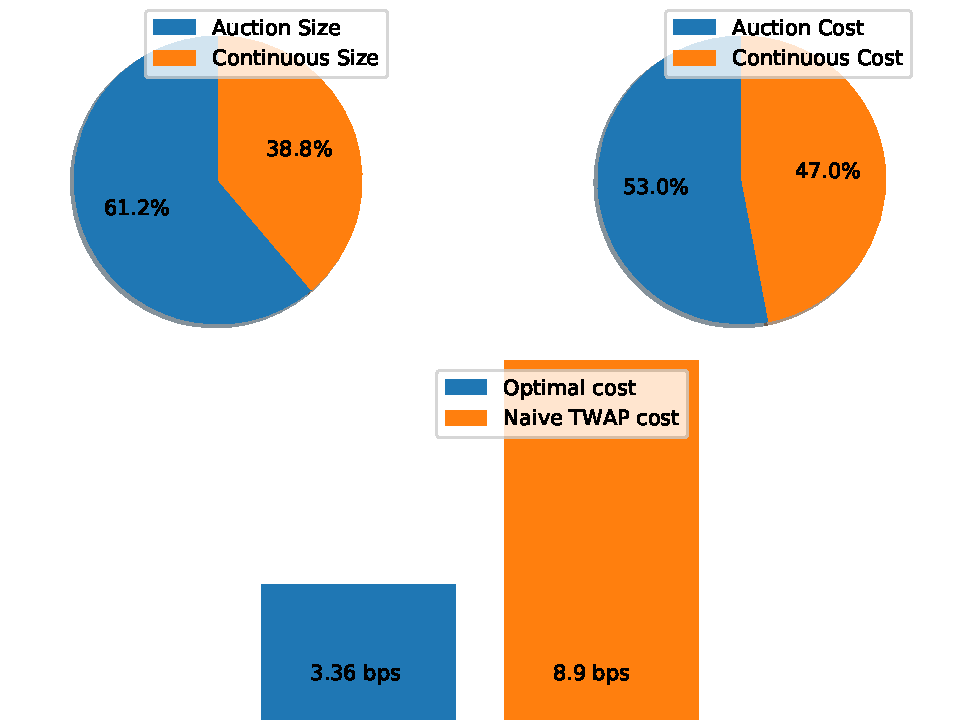
\includegraphics[width=\textwidth]{SampleTradeSize}
  \caption{Sample allocation between auction's block trade and the continuous trading strategy's size, using data from stock ACGL in October 2019, trading 5 percents of average trading volume of the first half of trading day. Compared to a pure TWAP trading stategy, the optimal stategy allocates 61.19 percents of the total position to be executed during the auction phase. The cost of trading in the auction phase accounts for 53.00 percents of the total cost of the strategy, while reducing 62.26 percents of total cost compared to a pure TWAP strategy, from 8.90 bps per share to 3.36 bps per share.}
  \label{fig:optimal_sizes}
\end{figure}



\begin{figure}[h]
  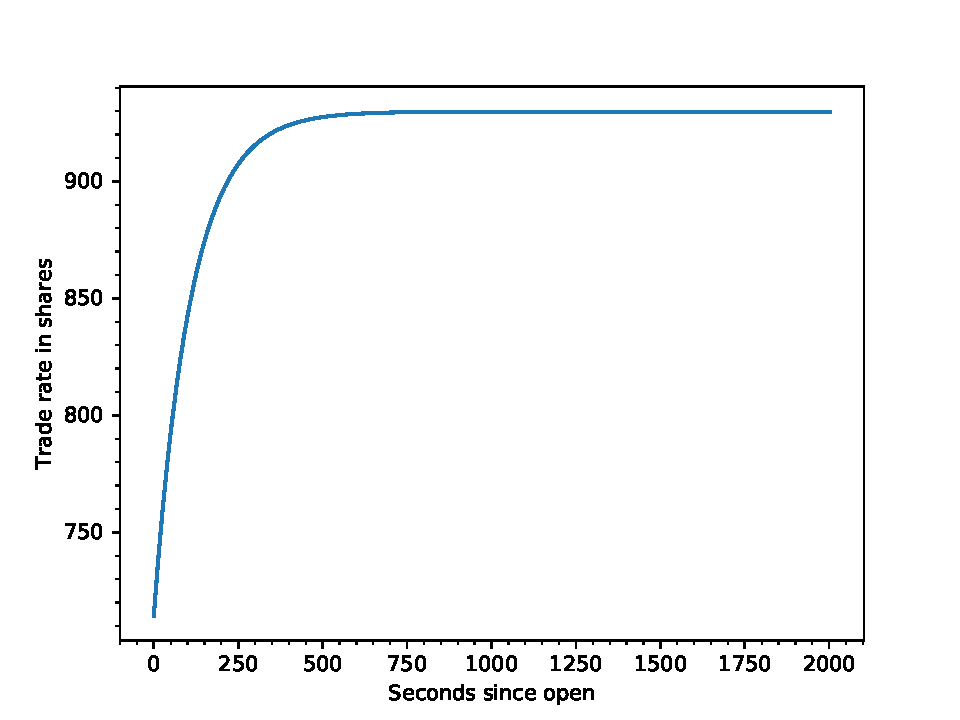
\includegraphics[width=\textwidth]{SampleTradeCurve}
  \caption{Sample optimal trading strategy's execution curve 30 minutes after market opens from auction phase. The shape of the optimal trading curve reflects the nature of the cost, in which the rate of execution is speed up over time as the market impact of the auction subsidizing and the spread narrowing.}
  \label{fig:optimal_curve_strategy}
\end{figure}

\subsection{Summary}

The main findings of this section can be summarized as follows:

\begin{itemize}
  \item The presence of informed trading from the market maker is required for the call auction to open, as the market maker will provide the necessary liquidity to offset the buy-sell imbalance at the end of the call auction.
  \item The transition period from the call auction will be characterized with a wide initial spread narrowing over time due to inventory management from the market maker.
  \item Trading in the call auction lower the cost of trading in general, as the call auction provides an additional venue for liquidity consumption.
  \item There is an optimal liquidation strategy to execute trade during both the call auction and the continuous auction. The mixing ratio of the strategy is determined by the efficiency of each auction, in terms of immediate cost of aggressing the book and the speed of spread recovery after market opening.
\end{itemize}

Before moving to empirical analysis, it is imperative to address some stylized facts of our model. We assume that the liquidity traders are price takers who submit market orders to signify his intention to trade regardless of opening price, and the market maker will post limit orders to counter the imbalance. In most modern stock exchanges, all participants can post limit orders in the order book to be "crossed" during the opening match. Limit orders can also be modified or cancelled before the opening match, allowing participants to update their pricing. However, as long as the market maker in our model can place his trade after all the liquidity traders has submitted their orders, the pricing schedule based on the market imbalance still holds.

We also assume that there is only one market maker and only he or she trades with private information. In practice, there can be multiple agents trading with information. However, as long as the private information is derived from public data, that is, no insider trading, we can assume that all informed agent will have the same "signal" regarding the fair price of the stock, and are only different in their risk aversion factor. Therefore, we can assume that all informed agents are trading with same risk aversion factor, which are represented by the market maker in our model.

The source of private information is also a vital assumption in our model. We assume that the market maker derives his valuation from public information, which include, but not limited to, the following factors:
\begin{itemize}
  \item Public order flow, with or without identity.
  \item General market information, such as index futures movement before equity market opening.
  \item Price continuity from previous day's closing price. In absence of any fundamental news, it is reasonable to expect the opening price to be close to the previous day's closing price.
\end{itemize}

Another deviation is the inventory management effects of the market maker. In our model, there is market maker's inventory management effects on the spread due to the position acquired from the opening auction, but not in the continuous auction. While it would be more complete to account for the inventory management effects in both auctions, our empirical analysis suggests that the inventory management effects of the continuous auction is less prominent compared to the opening auction. Specifically, we observed that
\begin{itemize}
  \item There is little evidence that the bid-ask spread is changed following a trade except near the opening and closing auctions.
  \item The auction matching volume is usually much larger than a normal trade during continuous phase, accounted for a significant fraction of the daily trading volume.
\end{itemize}

Last but not least, although it is immaterial to our cost analysis, it is not obvious that the market maker will make profit after placing his "stabilization" trade to counter the opening auction's imbalance. Even when his initial signal is correct up to the end of the opening auction, new information may come and he has to change his valuation of the stock before realize the gain from the call auction. This is evident in the high volatility immediately after market opening. However, the continuous book is only one of many execution venue for the market maker to realize his gain. For example, the market maker may attempt to "lock-in" his profit by hedging into the index futures immediately. He then can slowly unwind both legs of the hedge over the course of the day, resulting in a tightening spread over time.

With those caveats in mind, we can proceed to the empirical analysis of NASDAQ data to estimate the liquidation cost of trading in both auctions compared to only during the continuous auction.

\section{Empirical Analysis}\label{sec:EmpiricalAnalysis}

In this section, we will estimate the liquidation cost of trading in both auction for 40 stocks in the NASDAQ exchange using historical data in October 2019. We begin the section with the exchange rules regarding opening call auction and continuous auction of the NASDAQ exchange. After which, we provide description of our data, including how our stocks are picked, and our estimation methodology. Lastly, we provide cross-sectional analysis of our stock portfolio to show how liquidation cost changes with respect to tick size of the stock.

\subsection{Opening auction and continuous auction of the NASDAQ exchange}

Opening auction is NASDAQ is called \textbf{Opening Cross}. While similar to the general call auction described in our model, there are certain subtle difference between our model and the NASDAQ's Opening Cross:
\begin{itemize}
  \item Before the opening bell at 9:30 EST, NASDAQ allows investors to submit orders to two different books: a continuous book and an opening cross book. Orders submitted to the continuous book will be matched immediately and disseminate in the market data feed. Orders submitted to the opening cross book will be withheld to be matched later and are not visible in the market data feed.
  \item At 9:30 EST, the opening cross book and the continuous book will be merged together to form a single book, and a Opening Cross price will be calculated based on the following three rules, similar to our Walrasian matching rule:
        \begin{itemize}
          \item Maximize the number of shares executed.
          \item Minimize the imbalance of Cross orders.
          \item Minimize the distance from the Nasdaq inside bid-ask midpoint.
        \end{itemize}
        Matched orders and total matching quantity from the Opening Cross will then be disseminated in the market data feed. Market is considered to be in the continuous trading phase at this point of time.
\end{itemize}

While the presence of the continuous book during the call auction period deviates from our assumption, it makes little difference in practice due to limited volume transacted during this period. On the other hand, the hidden nature of the Opening Cross orders mean that we cannot directly derive the cost of aggressing the book during the call auction. Fortunately, based on the arguments in subsection (\ref{subsec:AnalyticalFrameworkTransitionPeriod}), we can infer the cost of trading during the call auction from the spread and matching volume immediate upon market opening.

The continuous auction in the NASDAQ exchange, on the other hand, is similar to our model.

\subsection{Data description}

Our data is captured directly from NASDAQ's ITCH-TotalView market data feed, provided by the National University of Singapore. The data contains all the add, modification, trade and delete for each order submitted to the continuous book, with fields indicating whether it is a buy or sell order. The data also contains the matching quantity and the Nasdaq Official Opening Price (NOOP) for each stock. Given the dataset of 3500 NASDAQ-listed stocks, we pick 40 random stocks with the following constraints:
\begin{itemize}
  \item Since we do not account for the value of the queue priority in our market maker's modelling, we avoid selecting stocks with tick size higher than 10 basis points in our sample.
  \item We avoid low liquidity stock by selecting ones higher than 10M daily traded notional, which is roughly the first quartile of our sample.
\end{itemize}

Given those constraints, we have the stock list in the Appendix, along with their sectors and fundamental statistics. Our analysis use 1 month of data, from 01/10/2019 to 31/10/2019. Since the intraday volumes usually follow a U-shaped pattern, we use the data from market opens at 9:30 EST to late noon at 12:00 PM in our analysis.

\subsection{Methodology}

In order to estimate the cost of trading, we need to estimate three factors:
\begin{itemize}
  \item The temporary book aggressing cost factor $\alpha$ before market opening in Equation (\ref{eqn:mm_eval_eqb})
  \item The temporary book aggressing cost factor $\beta$ during the continuous phase in Equation (\ref{eqn:mm_eval_cont})
  \item The spread recovery factor $\rho$ post opening auction in Equation (\ref{eqn:recovery_term_eqb})
\end{itemize}

We will describe our estimation methodology for each factors in the following.

\subsubsection{Estimation of cost factor $\alpha$}

Based on Equation (\ref{eqn:expected_spread}), we can estimate the coefficient $b_e$ as
\[
  \hat{b_e} = \frac{\bar{V_e}}{\bar{\zeta_e}}
\]
where
\begin{itemize}
  \item $\bar{V_e}$ is the average matching volume at the open.
  \item $\bar{\zeta_e}$ is the average spread at the open.
\end{itemize}

The estimation of cost factor $\alpha$ will then be
\[
  \hat{\alpha} = \frac{1}{\hat{b_e}}
\]

\subsubsection{Estimation of cost factor $\beta$}

Equation (\ref{eqn:markup_px_cont}) allows us to estimate cost factor $\beta$ directly from the liquidity posted in the book, with a slight adjustment. Since Equation (\ref{eqn:markup_px_cont}) is in terms of average price, we need to convert the price of the book to average price from the best bid-offer level, as illustrated in Table (\ref{tbl:bookAvgPxConversion}). Given the cumulative sum quantity as the independent variable $X$ and the average price as dependent variable $Y$, we have the $\beta$ estimate in a linear regression equation

\[
  Y_t = const + \beta * X_t + e_t
\]

One caveat is the period of observation for the regression. Given the discussion in Subsection (\ref{subsec:AnalyticalFrameworkTransitionPeriod}), we would want to avoid the transition period immediately after the opening. To identify this period, we perform two-sample t-test on consecutive 5-minute bin of data to determine if the average spread has stabilize. Specifically, given $\zeta_t$ as the average spread of the current bin and $\zeta_{t+1}$ as the average spread of the next 5-minute bin, the null hypothesis is:
\[
  H_0: \zeta_t = \zeta_{t+1}
\]
where the sample statistics of the spread mean is calculated as
\[
  \bar{\zeta_t} = \frac{\sum_{i=1}^N  \sum_{j=1}^5 \zeta_{ij}}{N*5}
\]
where $N$ is the number of days in our sample, and we measure the spread $\zeta_{ij}$ every 1 minute in each of the 5-minute bin. When we find the first 5-minute bin that we cannot reject the null hypothesis at $5 \%$ confidence level, we use the data in the bin as data for the regression. The sample statistics for $X$ and $Y$ is estimated similarly to the spread mean, where we bootstrap the average of 1-minute interval spread and cumulative sum quantity of the bin as sample data point. Furthermore, we use the data in the identified transition period to measure the recovery speed of the spread in the next subsection.

\begin{table}[h]
  \centering
  \begin{tabular}{c|c|c|c|l}
    \hline
    \textbf{Buy} & \textbf{Price} & \textbf{Sell} & \textbf{Sum} & \multicolumn{1}{c}{\textbf{Average Price}} \\ \hline
                 & 56             & 4000          & 14000        & 55.286                                     \\ \hline
                 & 55             & 10000         & 10000        & 55                                         \\ \hline
    900          & 54             &               & 900          & 54                                         \\ \hline
    100          & 53             &               & 1000         & 53.9                                       \\ \hline
    4000         & 52             &               & 5000         & 52.317                                     \\ \hline
  \end{tabular}
  \caption{A sample orderbook with average price calculated for each level. For example, the average price of the offer level 56 is $(55*10000+56*4000)/14000 = 55.286$}.
  \label{tbl:bookAvgPxConversion}
\end{table}

\subsubsection{Estimation of spread recovery factor $\rho$}

Given the transition period, we measure the average spread on a 1-minute interval:
\[
  \bar{\zeta_j} = \frac{\sum_{i=1}^N p_i}{N}
\]
where $j$ is the index of 1-minute interval, and $N$ is number of days in our dataset. From the time series $p_j$ we can perform an exponential linear regression to estimate $\rho$. We consider the following exponential model:
\[
  y = \theta e^{-\rho t}
\]
where the independent variable $t$ is number of seconds since market opening, and the dependent variable $y$ represented the average spread $\bar{\zeta_j}$.

\subsection{Summary}

The histogram of the cost saving percentage by using our optimal trading strategy over a TWAP is in Figure (\ref{fig:hist_cost_saving}), and the corresponding 5-number summary is in Table (\ref{table:CostSavingSummary}). From the significant cost saving presents across the board, we can conclude that our optimal trading strategy yields significant cost saving compared to a TWAP in continuous phase only. Since our sample represents a wide range of stocks in terms of tick size, market cap and sectors, as can be seen in Table \ref{table:StockBasics} and Figure (\ref{}), it is reasonable to assume a similar cost saving effects are present in other stocks in the market.

The cost factors, along with their standard deviation, is in Table (\ref{table:StockFactors}) in the Appendix. The cost breakdown and comparison to an equivalent TWAP strategy is in Table (\ref{table:StockCost}) in the Appendix.

\begin{figure}[h]
  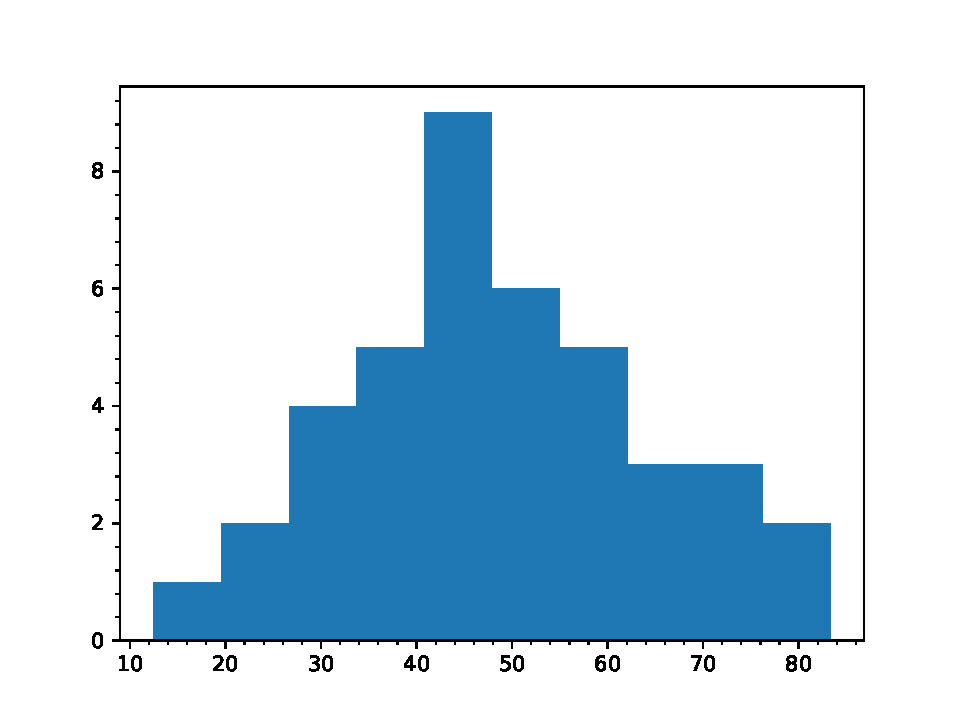
\includegraphics[width=\textwidth]{CostSavingChart}
  \caption{The histogram of the cost saving by using optimal trading stategy over a TWAP in percentage points. The saving percentage is significant across the stocks in our sample.}
  \label{fig:hist_cost_saving}
\end{figure}

\begin{figure}[h]
  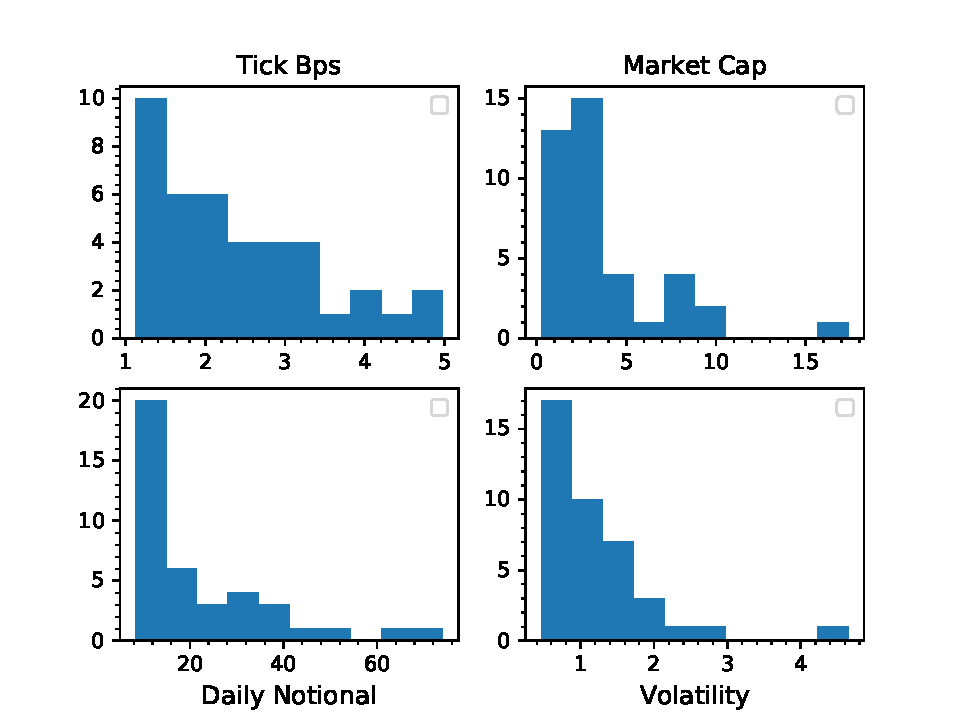
\includegraphics[width=\textwidth]{StockBasicsHist}
  \caption{Histogram of basic information of the stocks in our sample. As can be seen from those metrics, our stocks span a wide range in terms on tick size, market capitalization, daily traded notional and daily volatility.}
  \label{fig:stock_basics}
\end{figure}

\begin{table}
\centering
\caption{5-number summary of the cost saving percentage by using the optimal tradings strategy against a TWAP strategy. Given the minimum is 12.50 percents and median is 40.13 percents, the saving percentage is significant across the stocks in our sample.
}
\label{table:CostSavingSummary}
\begin{tabular}{lllll}
\toprule
Median & 1st Quartile & 3rd Quartile & Minimum & Maximum \\
\midrule
 47.66 &        40.13 &        56.71 &   12.50 &   83.30 \\
\bottomrule
\end{tabular}
\end{table}



\section{Conclusion}\label{secConclusion}
We shows that when the cost of trading in the call auction is comparable to the continuous trading phase, our strategy yields significant cost savings. Subsequent research on different forms of market impact under both auctions, and extending to multi-phase auction market, can be conducted in the future to yield more interesting findings.

\section{Appendix}

\begin{table}
\centering
\caption{Basic information of the stocks in our sample. Descriptions of each columns are: \\
 * \textbf{Symbol}: The abbreviation used to uniquely identify publicly traded shares of the company on NASDAQ. \\
 * \textbf{Company Name}: The name of the company. \\
 * \textbf{Sector}: The sector of the stock based on the Bloomberg Industry Classification Systems (BICS). \\
 * \textbf{Market Cap}: The total market capitalization of the stock, measured in billions of USD. \\
 * \textbf{Daily Notional}: The average daily traded notional of the stock, measured in millions of USD. \\
 * \textbf{Volatility}: The daily volatility of the stock, measured in percentage points. \\
 * \textbf{Tick Bps}: The ratio of the tick size of the stock over its average price, measured in basis points.\\
}
\label{table:stockBasicsTable}
\begin{tabular}{lllrrrr}
\toprule
Symbol &      Company Name &                       Sector &  Market Cap &  Daily Notional &  Volatility &  Tick Bps \\
\midrule
  SKYW &       SKYWEST INC &                     Airlines &        3.25 &           11.15 &        1.03 &      1.72 \\
  MNRO &         MONRO INC &          Auto Repair Centers &        1.33 &           25.01 &        1.99 &      1.27 \\
  FFIN &  FIRST FIN BANKSH &      Commer Banks-Central US &        4.74 &           12.43 &        0.52 &      3.11 \\
  BOKF &     BOK FINL CORP &      Commer Banks-Central US &        6.62 &           12.01 &        1.41 &      1.28 \\
  CBSH &    COMMERCE BCSHS &      Commer Banks-Central US &        7.63 &           27.88 &        0.76 &      1.68 \\
  COLB &  COLUMBIA BANKING &      Commer Banks-Western US &        2.93 &            9.34 &        0.55 &      2.77 \\
  CATY &  CATHAY GENERAL B &      Commer Banks-Western US &        3.03 &           12.39 &        0.56 &      2.87 \\
  JCOM &     J2 GLOBAL INC &            Computer Software &        4.47 &           29.63 &        1.14 &      1.13 \\
  CVLT &  COMMVAULT SYSTEM &         Data Processing/Mgmt &        1.86 &           21.49 &        0.92 &      2.18 \\
  EPAY &   BOTTOMLINE TECH &         Data Processing/Mgmt &        2.14 &           10.00 &        0.67 &      2.42 \\
  CORE &  CORE-MARK HOLDIN &       Distribution/Wholesale &        1.23 &            8.41 &        0.69 &      3.01 \\
  NOVT &       NOVANTA INC &       Electric Products-Misc &        3.10 &           12.01 &        1.65 &      1.22 \\
  PLXS &       PLEXUS CORP &        Electronic Compo-Misc &        1.81 &            9.91 &        1.23 &      1.64 \\
  SANM &      SANMINA CORP &        Electronic Compo-Misc &        2.24 &           11.35 &        0.59 &      3.25 \\
  MTSI &  MACOM TECHNOLOGY &     Electronic Compo-Semicon &        1.43 &           11.98 &        0.55 &      4.98 \\
  ALRM &  ALARM.COM HOLDIN &     Electronic Secur Devices &        2.09 &           16.66 &        0.85 &      2.06 \\
  MANT &    MANTECH INTL-A &     Enterprise Software/Serv &        3.21 &            9.17 &        1.37 &      1.45 \\
  MANH &   MANHATTAN ASSOC &     Enterprise Software/Serv &        5.06 &           42.92 &        1.96 &      1.24 \\
  NMIH &  NMI HOLDINGS I-A &      Financial Guarantee Ins &        2.27 &           12.15 &        0.61 &      3.64 \\
  JBSS &  JOHN B SANFILIPP &        Food-Misc/Diversified &        0.94 &            8.34 &        1.86 &      1.12 \\
  CCOI &  COGENT COMMUNICA &      Internet Connectiv Svcs &        3.08 &           15.75 &        1.00 &      1.70 \\
  SINA &         SINA CORP &   Internet Content-Info/News &        2.73 &           32.98 &        1.08 &      2.46 \\
  BRKR &       BRUKER CORP &          Medical Instruments &        7.86 &           33.24 &        0.85 &      2.25 \\
  NSTG &  NANOSTRING TECHN &             Medical Products &        1.01 &           12.03 &        0.89 &      3.97 \\
  NVCR &      NOVOCURE LTD &             Medical Products &        8.39 &           62.22 &        2.37 &      1.27 \\
  HSIC &  HENRY SCHEIN INC &             Medical Products &        9.54 &           74.05 &        0.87 &      1.56 \\
  ANIP &  ANI PHARMACEUTIC &      Medical-Biomedical/Gene &        0.75 &           11.65 &        1.56 &      1.34 \\
  MYGN &   MYRIAD GENETICS &      Medical-Biomedical/Gene &        0.85 &           34.78 &        2.82 &      3.39 \\
  ALLK &       ALLAKOS INC &      Medical-Biomedical/Gene &        4.02 &           39.51 &        4.65 &      1.47 \\
  AIMT &  AIMMUNE THERAPEU &                Medical-Drugs &        2.13 &           20.50 &        0.81 &      4.61 \\
  MYOK &     MYOKARDIA INC &                Medical-Drugs &        3.38 &           14.74 &        1.39 &      1.86 \\
  MLHR &     HERMAN MILLER &      Office Furnishings-Orig &        1.35 &           18.87 &        0.66 &      2.25 \\
   PPC &   PILGRIM'S PRIDE &                      Poultry &        8.23 &           31.04 &        0.58 &      3.42 \\
  JRVR &  JAMES RIVER GROU &        Property/Casualty Ins &        1.25 &            8.96 &        1.30 &      2.15 \\
  ACGL &  ARCH CAPITAL GRP &        Property/Casualty Ins &       17.40 &           50.32 &        0.46 &      2.50 \\
  CONN &        CONN'S INC &            Retail-Appliances &        0.25 &           12.00 &        0.72 &      4.51 \\
  BJRI &  BJ'S RESTAURANTS &           Retail-Restaurants &        0.73 &           18.42 &        1.26 &      2.62 \\
  AFYA &  AFYA LTD-CLASS A &                      Schools &        9.78 &           10.66 &        1.40 &      3.88 \\
  CRUS &  CIRRUS LOGIC INC &  Semicon Compo-Intg Circuits &        3.61 &           36.46 &        1.65 &      1.91 \\
  BRKS &  BROOKS AUTOMATIO &      Semiconductor Equipment &        2.68 &           15.38 &        1.05 &      2.70 \\
\bottomrule
\end{tabular}
\end{table}



\begin{table}
\centering
\caption{Estimated params for the optimal trading strategy. Descriptions of each columns are: \\
 * \textbf{Auction Factor}: The temporary book aggressing cost factor $\alpha$ before market opening. Unit is basis point per share.\\
 * \textbf{Continuous Factor}: The temporary book aggressing cost factor $\beta$ during the continuous phase. Unit is basis point per share.\\
 * \textbf{Recovery Rate}: The spread recovery factor $\rho$ post opening auction. Unit is percentage points per second.\\
}
\label{table:StockFactors}
\begin{tabular}{llll}
\toprule
Symbol & Auction Factor & Continuous Factor &  Recovery Rate \\
\midrule
  ACGL &  0.004 (0.002) &     0.007 (0.004) &  0.004 (0.003) \\
  AFYA &  1.206 (0.829) &     0.157 (0.072) &  0.087 (0.089) \\
  AIMT &  0.013 (0.011) &     0.050 (0.023) &  0.009 (0.005) \\
  ALLK &  0.246 (0.173) &     0.163 (0.087) &  0.031 (0.019) \\
  ALRM &  0.095 (0.066) &     0.089 (0.036) &  0.010 (0.006) \\
  ANIP &  0.361 (0.424) &     0.148 (0.071) &  0.019 (0.012) \\
  BJRI &  0.057 (0.035) &     0.058 (0.019) &  0.020 (0.010) \\
  BOKF &  0.345 (0.190) &     0.169 (0.088) &  0.021 (0.013) \\
  BRKR &  0.048 (0.029) &     0.041 (0.015) &  0.011 (0.006) \\
  BRKS &  0.045 (0.035) &     0.057 (0.015) &  0.013 (0.006) \\
  CATY &  0.067 (0.039) &     0.058 (0.013) &  0.021 (0.029) \\
  CBSH &  0.025 (0.015) &     0.035 (0.012) &  0.010 (0.006) \\
  CCOI &  0.099 (0.060) &     0.089 (0.032) &  0.015 (0.008) \\
  COLB &  0.065 (0.029) &     0.059 (0.026) &  0.029 (0.029) \\
  CONN &  0.050 (0.021) &     0.052 (0.019) &  0.015 (0.008) \\
  CORE &  0.093 (0.040) &     0.078 (0.027) &  0.036 (0.028) \\
  CRUS &  0.023 (0.021) &     0.038 (0.011) &  0.010 (0.006) \\
  CVLT &  0.046 (0.030) &     0.052 (0.014) &  0.013 (0.009) \\
  EPAY &  0.140 (0.094) &     0.093 (0.026) &  0.023 (0.011) \\
  FFIN &  0.038 (0.036) &     0.047 (0.016) &  0.012 (0.007) \\
  HSIC &  0.013 (0.016) &     0.012 (0.003) &  0.006 (0.003) \\
  JBSS &  0.410 (0.305) &     0.119 (0.051) &  0.030 (0.013) \\
  JCOM &  0.072 (0.119) &     0.053 (0.020) &  0.012 (0.009) \\
  JRVR &  0.267 (0.279) &     0.120 (0.054) &  0.023 (0.013) \\
  MANH &  0.069 (0.038) &     0.057 (0.023) &  0.010 (0.004) \\
  MANT &  0.317 (0.210) &     0.133 (0.042) &  0.035 (0.019) \\
  MLHR &  0.017 (0.011) &     0.038 (0.015) &  0.008 (0.004) \\
  MNRO &  0.165 (0.127) &     0.084 (0.035) &  0.023 (0.012) \\
  MTSI &  0.041 (0.028) &     0.047 (0.009) &  0.013 (0.005) \\
  MYGN &  0.028 (0.015) &     0.060 (0.019) &  0.011 (0.007) \\
  MYOK &  0.144 (0.081) &     0.115 (0.043) &  0.024 (0.012) \\
  NMIH &  0.015 (0.008) &     0.042 (0.018) &  0.015 (0.010) \\
  NOVT &  0.539 (0.491) &     0.134 (0.057) &  0.027 (0.021) \\
  NSTG &  0.111 (0.063) &     0.075 (0.018) &  0.021 (0.009) \\
  NVCR &  0.011 (0.007) &     0.053 (0.027) &  0.007 (0.004) \\
  PLXS &  0.293 (0.294) &     0.147 (0.065) &  0.024 (0.015) \\
   PPC &  0.010 (0.006) &     0.020 (0.009) &  0.008 (0.005) \\
  SANM &  0.046 (0.033) &     0.057 (0.022) &  0.013 (0.006) \\
  SINA &  0.015 (0.007) &     0.040 (0.016) &  0.006 (0.002) \\
  SKYW &  0.123 (0.077) &     0.097 (0.033) &  0.018 (0.013) \\
\bottomrule
\end{tabular}
\end{table}



\begin{table}
\centering
\caption{Cost and trade quantity breakdown of the optimal strategy, with comparision to a naive TWAP strategy. Descriptions of each columns are: \\
 * \textbf{Auction Qty}: Number of shares traded in the opening call auction in the optimal strategy. Unit is basis point per share. \\
 * \textbf{Auction Cost}: The cost of the call auction session's portion in the optimal strategy. Unit is basis point per share. \\
 * \textbf{Continuous Qty}:  Number of shares traded in the continuous phase in the optimal strategy. \\
 * \textbf{Continuous Cost}: The cost of the continuous session's portion in the optimal strategy. Unit is basis point per share. \\
 * \textbf{Optimal Cost}: The total cost of the optimal strategy. Unit is basis point per share. \\
 * \textbf{TWAP Cost}: The total cost of an equivalent naive TWAP strategy. Unit is basis point per share. \\
 * \textbf{Cost Saving}: The percentage difference in total cost between using the optimal strategy and the naive TWAP strategy. Unit is percentage point.\\
}
\label{table:StockCost}
\begin{tabular}{lrrrrrrr}
\toprule
Symbol &  Auction Qty &  Auction Cost &  Continuous Qty &  Continuous Cost &  Optimal Cost &  TWAP Cost &  Cost Saving \\
\midrule
  ACGL &       687.43 &          1.78 &          436.06 &             1.58 &          3.36 &       8.90 &        62.26 \\
  AFYA &         7.77 &          1.07 &           60.22 &             9.34 &         10.41 &      11.90 &        12.50 \\
  AIMT &       793.84 &          8.31 &          216.43 &             2.59 &         10.89 &      51.57 &        78.87 \\
  ALLK &        67.66 &          6.60 &          102.91 &            11.02 &         17.62 &      29.43 &        40.14 \\
  ALRM &        97.31 &          4.43 &          106.35 &             5.72 &         10.15 &      19.70 &        48.47 \\
  ANIP &        20.69 &          2.15 &           51.27 &             6.38 &          8.53 &      12.16 &        29.86 \\
  BJRI &       253.74 &          7.25 &          249.75 &             7.72 &         14.97 &      30.38 &        50.74 \\
  BOKF &        26.35 &          2.96 &           54.40 &             6.95 &          9.91 &      14.87 &        33.36 \\
  BRKR &       143.11 &          3.13 &          171.51 &             4.47 &          7.60 &      14.13 &        46.25 \\
  BRKS &       199.37 &          4.96 &          159.48 &             4.54 &          9.51 &      21.63 &        56.04 \\
  CATY &       120.26 &          3.72 &          138.54 &             4.89 &          8.61 &      16.25 &        47.03 \\
  CBSH &       273.67 &          3.97 &          197.28 &             3.40 &          7.37 &      17.85 &        58.72 \\
  CCOI &        78.69 &          3.67 &           88.57 &             4.89 &          8.57 &      16.39 &        47.74 \\
  COLB &       127.75 &          3.92 &          143.21 &             4.86 &          8.77 &      16.73 &        47.58 \\
  CONN &       166.65 &          4.23 &          160.46 &             4.59 &          8.82 &      18.17 &        51.43 \\
  CORE &       116.47 &          4.93 &          140.32 &             6.48 &         11.41 &      21.04 &        45.76 \\
  CRUS &       429.80 &          6.12 &          270.41 &             4.63 &         10.75 &      28.28 &        61.98 \\
  CVLT &       231.18 &          5.64 &          209.68 &             5.99 &         11.62 &      24.75 &        53.03 \\
  EPAY &        80.80 &          4.48 &          123.45 &             7.59 &         12.07 &      20.14 &        40.09 \\
  FFIN &       222.49 &          4.65 &          185.60 &             4.62 &          9.27 &      20.67 &        55.15 \\
  HSIC &       480.48 &          2.98 &          530.39 &             4.49 &          7.46 &      14.57 &        48.76 \\
  JBSS &        16.81 &          1.54 &           58.54 &             6.20 &          7.73 &      10.09 &        23.34 \\
  JCOM &       101.54 &          3.09 &          139.41 &             5.20 &          8.30 &      14.57 &        43.07 \\
  JRVR &        50.59 &          4.16 &          113.85 &            10.99 &         15.15 &      22.18 &        31.71 \\
  MANH &       137.68 &          4.23 &          169.90 &             6.10 &         10.33 &      18.94 &        45.47 \\
  MANT &        36.05 &          3.35 &           86.99 &             8.93 &         12.28 &      17.52 &        29.92 \\
  MLHR &       275.38 &          3.18 &          124.64 &             1.80 &          4.97 &      16.25 &        69.39 \\
  MNRO &        58.57 &          3.24 &          116.14 &             7.41 &         10.65 &      16.22 &        34.32 \\
  MTSI &       296.63 &          6.46 &          266.15 &             6.69 &         13.15 &      28.13 &        53.26 \\
  MYGN &       357.58 &          6.73 &          167.36 &             3.65 &         10.38 &      32.99 &        68.52 \\
  MYOK &        77.80 &          4.96 &           97.97 &             6.90 &         11.85 &      21.44 &        44.72 \\
  NMIH &       419.55 &          4.53 &          146.55 &             1.83 &          6.37 &      24.89 &        74.42 \\
  NOVT &        18.19 &          1.94 &           73.90 &             9.25 &         11.19 &      14.16 &        20.96 \\
  NSTG &       106.11 &          4.74 &          158.66 &             8.07 &         12.81 &      21.61 &        40.72 \\
  NVCR &       542.87 &          4.76 &          111.58 &             1.22 &          5.98 &      35.81 &        83.30 \\
  PLXS &        45.64 &          4.43 &           92.49 &            10.33 &         14.75 &      22.30 &        33.84 \\
   PPC &       586.45 &          3.79 &          296.53 &             2.35 &          6.14 &      18.60 &        67.01 \\
  SANM &       196.35 &          4.96 &          159.26 &             4.73 &          9.69 &      21.92 &        55.78 \\
  SINA &       390.33 &          4.24 &          150.11 &             1.98 &          6.22 &      22.82 &        72.73 \\
  SKYW &        68.74 &          3.70 &           88.29 &             5.49 &          9.19 &      16.54 &        44.43 \\
\bottomrule
\end{tabular}
\end{table}



\begin{proof}[Derivation of the optimal trading strategy]\label{proof:optimal-strategy}
  The cost of trading in both auction given the notations in the paper is:
  \[
    C = \alpha B_0^2  + \alpha \int_0^T \frac{B_0 + V_e}{2} e^{-\rho s} E_s ds + \beta \int_0^T E_s^2 ds
  \]

  We need to find a tuple of $(B_0, E_t, X_t)$ as a stationary point (function) of the functional. First we assume $B_0$ is static, and solve the cost of trading during continuous phase:
  \[
    C_c = \int_0^T \frac{B_0 + V_e}{2} \alpha e^{-\rho s} E_s ds + \int_0^T  \beta E_s^2 ds
  \]
  which has the following Euler-Lagrange equation
  \[
    \frac{\alpha}{4 \beta} B_0  e^{-\rho s} +E_s = A
  \]
  \[
    \Leftrightarrow \hat{E_s} = A - \frac{\alpha}{4 \beta} B_0 e^{-\rho s}
  \]
  \[
    \Leftrightarrow \hat{X_t} = At + B - \frac{\alpha}{4 \beta \rho}B_ 0 (1 - e^{-\rho t})
  \]
  Using the boundary conditions:
  \[
    \hat{X_0} = 0
  \]
  \[
    \hat{X_T} = Q_0 - B_0
  \]
  we have
  \[
    B = 0
  \]
  \[
    A = \frac{4 (Q_0 - B_0) + \frac{(1 - e^{-T \rho})}{\beta \rho} B_0 \alpha} {4 T}
  \]
  Taking the first derivative of the cost function $C$ w.r.t. $B_0$ and solve for $B_0$, we have
  \[
    B_0 = \frac{Q_0 F_{11} + V_e F_{12}}{F_2}
  \]
  where
  \[
    F_{11} = 8 e^{T \rho} \beta \rho [\alpha - e^{T \rho} (\alpha - 4 \beta \rho)]
  \]
  \[
    F_{12} = (e^{T \rho}-1) \alpha [\alpha (2+T \rho) + e^{T \rho} (8 \beta \rho + \alpha (T \rho - 2 ))]
  \]
  \[
    \begin{split}
      F_2 = \alpha^2 (2 + T \rho) - 4 e^{T \rho} \alpha (\alpha + 2 \beta \rho)
      + e^{2 T \rho} [8 \beta \alpha \rho + 8 \beta (T \alpha + \beta) \rho^2 + \alpha^2 (2 - T \rho)]
    \end{split}
  \]

\end{proof}

\bibliographystyle{plain}
\bibliography{references}
\end{document}

